\section{Optimization}
To maximize cumulative discounted profit in a framework of NaaA,
it is important to balance the two contradicting criteria, revenue $r_{it}$ and cost $c_{it}$.

%TODO: 否定的な結論。何が問題か。

%\begin{thm}\label{thm:optimal-bidding-simple}
%	The Nash equivalem of the game $(r_{ijt})$ is $0$.
%\end{thm}
%ただちに、次の系が成立する。
%\begin{coro}\label{coro:optimal-bidding-simple}
%NaaA では、外的環境から報酬を受け取らないニューロンはすべて NOOP になる。
%\end{coro}

To achieve that, we employ mechanism design.
The reason why we introduce mechanism design is, unlike the several existing studies \citep{sukhbaatar2016learning}, NaaA assumes all the agent is not cooperative but selfish.
%(TODO: このあたりの文章は要検討)
If we naively optimize the optimization problem of NaaA, we obtain the trivial solution that the internal rewards will converges to 0, and all the units becomes NOOP.
Hence, the multi-agent system should select the action without any information, and it is equivalent to take an action randomly.
Therefore, the external reward $R_t^{\mathrm ex}$ shrinks obviously.

%これは、ナッシュ均衡がパレート最適と一致しないパレート劣位な状況が発生する。

\subsection{Envy-free Auction}
To achieve the Pareto optimality, we borrow the idea from digital goods auction.
The auction theory belongs mechanism design, and it towards to unveil the true price of the goods.
Digital goods auction is one of the mechanism from auction theory,
and it is target to copyable goods without cost such as digital book and music.

Although there are several variation of digital goods auction,
we use envy-free auction \citep{guruswami2005profit} because it requires simple assumption.
The assumption is same goods have one price at the same time.
In NaaA, it can be represented as the following assumption:
\begin{enumerate}
\renewcommand{\labelenumi}{N\arabic{enumi}:}
\setcounter{enumi}{4}
\item (Law of one price)
	If $\rho_{j_1,i,t}, \rho_{j_2,i,t} > 0$, then $\rho_{j_1,i,t} = \rho_{j_2,i,t}$.
\end{enumerate}
It means that $\unit$ has an intrinsic price at the same timing $t$.
We denote the price as $q_{it}$.

\begin{figure*}[t]
\centering
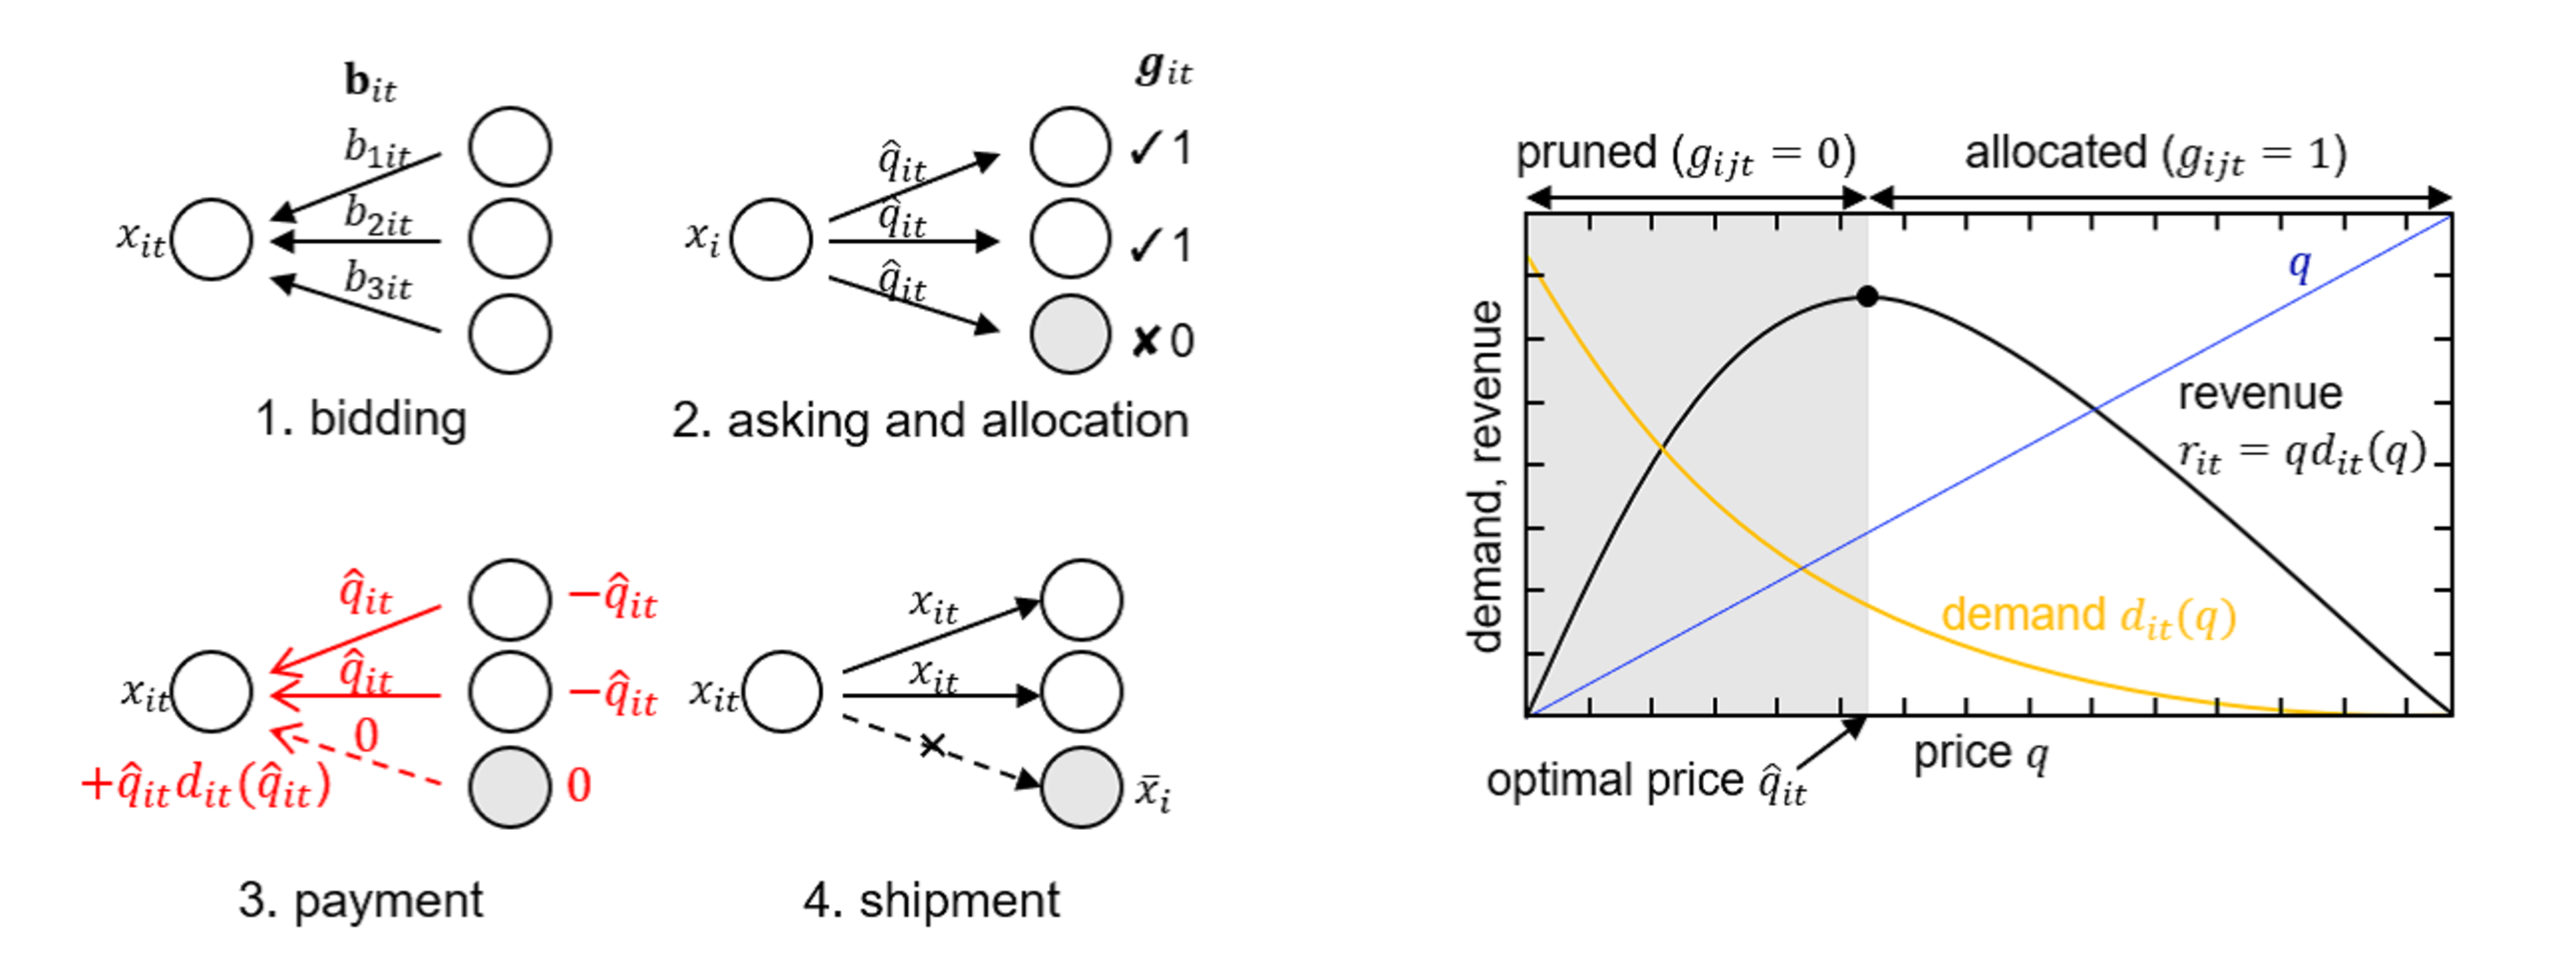
\includegraphics[width=\linewidth]{img/double.eps}
\caption{
\textbf{Left}: the process of trade in envy-free auction.
\textbf{Right}: a price determination curve for a unit. Revenue of a unit is a product of monotonically decreasing demand and price, and the price maximizing the revenue is the optimal price.
}
\label{fig:double}
\end{figure*}

% TODO 割当の話
We show the process of envy-free auction in left of Figure \ref{fig:double}.
It shows the negotiation process between one unit in sending activation and a group of units which buy the activation.
The negotiation performed per time step in RL.
We name the unit in sending activation as a seller, and units in buying activation as a buyer.
First, the buyer bid the unit in bidding price $b_{jit}$ (\textbf{1}).
Next, the seller decides the optimal price $\opt{q}_{it}$, and perform allocation (\textbf{2}).
After allocation, the buyers perform payment as $\rho_{jit} = g_{jit} \opt{q}_{it}$ (\textbf{3}), and
the seller only send the activation $x_i$ to the allocated buyers (\textbf{4}).
The buyer which cannot receive the activation approximates $x_i$ with $\Expect{\pi}{x_i}$.

In the following, we discuss of revenue, cost and value function based on Eq:(\ref{eq:V}).

%以下では、Envy-free auction における収益 $r_{it}$ とコスト $c_{it}$ の最適化について分けて説明を行う。

%この過程は、本や音楽などの、複製可能財、digital goods を対象にしたオークション理論 digital goods auction において、
%envy-free auction として知られている。
%後で示すように、このシンプルな前提のみでジレンマの問題が解決する。
%NaaA による取引の流れを図\ref{fig:double}に示す。

%========================================
% 収益
%========================================

\textbf{Revenue}:
The revenue of a unit is given as the following equaiton:
\begin{flalign}
	r_{it}  &= \sum_{j \in N^\mathrm{out}_i} g(b_{jit}, q_{it}) q_{it} + R^\mathrm{ex}_i  = q_{it} \sum_{j \in N^\mathrm{out}_i} g(b_{jit}, q_{it})  + R^\mathrm{ex}_i \notag \\
		&= q_i d_{it}(q_t) + R^\mathrm{ex}_i,
\end{flalign}
where $g(\cdot, \cdot)$ is allocation, and defined using a step function $H(\cdot)$ as $g(b,q)=H(b - q)$.
$d_{it}(q_{it})$ is a count of units which the bidding price for $q_{it}$ is more than or equal to $q_{it}$, and named as demand.
$q_{it}$ maximizing the equation is named as the optimal price, and denoted as $ \opt{q}_{it} $.
As the second term in the equation is independent of $q_t$, the optimal price $\opt{q}_{it}$ is given as the following euqaiton.
\begin{flalign}
	\opt{q}_{it}  = \argmax_{q \in [0, \infty)} q d_{it}(q).
\end{flalign}
We illustrate the curve of $q_{it}$ in the right side of Figure \ref{fig:double}.


%========================================
% コスト
%========================================
\textbf{Cost}:
The cost is internal reward which the unit should pay to other units,
and it is represented by the following equation:
\begin{flalign}
	c_{it} = \sum_{j \in N^\mathrm{in} } g(b_{ijt}, q_j) q_j
\end{flalign}
Although $c_{it}$ itself is minimized when $b_{ijt} = 0$,
this has trade-off with the next value function.

\textbf{Value Function}:
%Value of the value function $V(s_{i,t+1})$ depends on $s_{i,t+1}$.
%As we already defined, the internal environment of $v_i$ is a set of connected units,
%and the output of units affect to evaluation from the units, namely, weight of edges.
%As the learning rule of a typical artificial neural network obeys to law of Hebb, 
%the reward becomes lower because weight of unit which do not contribute
%the accuracy of output becomes lower.
Activation $x_i$ depends on the input from the units in $N_i^{\mathrm in}$, and affects to bidding price from units in $N_i^{\mathrm out}$.
If we minimize $b_{ijt}$ and let $b_{ijt} = 0$, then the purchase of activation fails, the reward can the unit can obtain from the units which 
the unit connect to becomes lower in the future.

Then, we denote the allocation as $\vect{g}_{it} = (g_{i1t}, \dots, g_{iNt})^\T$, 
and consider effect for value function in the cases when an unit succeed to purchase $v_j$ or not.
The value function can be written as the equation using state-value function $Q(s_{i,t+1}, \vect{g}_{i,t+1})$.
\begin{flalign}
	V_i^{\pi_i}(s_{it}) 
	&= Q_i^{\pi_i}(s_{it}, \vect{g}_{it}) \notag \\
	&= \sum_{j \in \followees} g_{ijt} (Q_i^{\pi_i} (s_{it}, \vect{e}_j) - Q_i^{\pi_i}(s_{it}, \vect{0})) + Q_i^{\pi_i}(s_{it}, \vect{0}) \notag \\
	&= \sum_{j \in \followees} g_{ijt} o_{ijt} + Q_i^{\pi_i}(s_{it}, \vect{0}) \notag \\
	&= \vect{g}_{it}^\T \vect{o}_{it} + Q_i^{\pi_i}(s_{it}, \vect{0})
\end{flalign}

We name $o_{ijt} = Q_i^{\pi_i} (s_{it}, \vect{e}_j) - Q_i^{\pi_i}(s_{it}, \vect{0})$ as {\em counterfactual return}, 
which is equivalent to cumulative discount value of counterfactual reward \citep{agogino2006quicr}.
That is, the cost the unit will pay is $\opt{q}_{it}$ in success of purchasing data, and $o_{it}$ otherwise.

Therefore, the optimization problem is below.
\begin{flalign}
	\max_{\vect{b}, q} \Expect{\hat{\vect{q}}_t}{ V_i^{\pi_i}(s_{it}) } = 
		\max_q q d_{it}(q) - 
		\min_{\vect{b}} \Expect{\hat{\vect{q}}_t}{\vect{g}_{it}(\vect{b})^\T( \hat{\vect{q}}_t - \gamma \vect{o}_{i,t+1}  )} + \const.
\end{flalign}
Note that we take expectation $\Expect{\hat{\vect{q}}_t}{\cdot}$ 
because the asked price $\hat{\vect{q}}_t$ is unknown for $v_i$ except of $\hat{q}_{it}$, and $g_{iit} = 0$.

Then, how much is bidding price $b_{it}$ to maximize return?
The following theorem holds.

\begin{thm}\label{thm:optimal-bidding}
	(Truthfulness) the optimal biding price maximizing return is $\opt{\vect{b}}_{it} = \vect{o}_{it}$.
\end{thm}
See Appendix for the proof.

That is, the unit should only consider its counterfactual return (!).
Hence, in the mechanism of NaaA, the unit obeys as if performing valuation to the other units, 
and declare the value truthfully.

Then, the corollary holds,
\begin{coro}\label{coro:optimal-bidding}
	The Nash equilibrium of an envy-free auction $(\vect{b}_{it}, q_{it})$ is $(\vect{o}_{it}, \argmax_{q} q d_{it}(q))$.
\end{coro}


%\subsection{Valuation Net}
%The remaining problem is how to predict $\vect{o}_t$,
%Although there are several prediction method for the issue, and we can apply a lot of methods, we employ $Q$-learning to predict $Q$.
%We note that we can alos use on-policy method such as actor-critic.
%
%A valuation net in Figure \ref{fig:network} is a network combining a typical unit 
%
%
%\subsection{Adaptive Dropconnect}
式に注目すると、この式はトポロジーを強化学習を用いて最適化しているように見える。

本研究では、方策として $\varepsilon$-greedy を用いる。
具体的に、adaptive dropconnectを用いる。




\iffalse
\subsection{Valuation Net}

\begin{figure*}[t]
\centering
\includegraphics[width=\linewidth]{img/network.eps}
\caption{
Valuationn Net は情報の価値を評価し、bidding price を決定する。
下位のニューロンに対して入札し、信号を購入する。購入したデータを用いて、データを次のニューロンに対して売る。
}
\label{fig:network}
\end{figure*}

残る問題は、$\vect{o}_t$ をいかに推定するかである。
この推定には様々な方法が存在しており、多くのメソッドを使うことができるが、
本論文では $Q$ の推定に $Q$-learning を採用する。
ただし、SARSA や actor-critic などの on-policy な方法も使うことができることを補足する。

図\ref{fig:network}に示すValuation Net は、通常のニューラルネットワークのユニットに、
$Q$-learning による valuation を組み合わせたネットワークである。
まず、上部はエージェント間の通信について示したものである。
ニューラルネットワークではユニットを円で表現するのが通例であるが、
ここではユニットをエージェントとしてみなすことを強調して、六角形で一つのユニットを表現している。
エージェント間では、通常のニューラルネットワークと同様の信号の通信以外に、
取引に関する通信(allocate, buy, sell \& bid)が発生する。

Valuation Net では、状態 $\vect{s}_t$ として、
予測後入力 $\tilde{\vect{x}}_t$ および入力に依存しない構成情報 $\vect{u}$ を横につなげたベクトル $(\tilde{\vect{x}}_t^\T, \vect{u}^\T)^\T$ を用いる。
構成情報の一例としてはユニットのパラメータがあげられ、たとえば重みやバイアスの情報を用いることができる。

状態からの Q 関数の予測にニューラルネットワークを用いる。
エージェントが受け取った収益に基づき時間差分(TD)-誤差 が計算され、
ネットワークが訓練される。
ネットワークの構成にはこれまでの deep Q-learning で用いられている二重化ネットワーク(dueling network) \citep{wang2015dueling} のテクニックを用いる。
オリジナルの文献\citep{wang2015dueling}で述べられている二重化ネットワークは、学習を加速するために、
状態関数と、Q関数との差分を別々に予測する手法である。
\cite{dosovitskiy2016learning} はこれに対して、差分の要素の総和が 0 になるように正規化するよう改良している。
本研究では \cite{dosovitskiy2016learning} の手法に従い、
期待値 $\edges(\vect{s}_t)$ と正規化差分 $\tilde{A}(\vect{s}_t)$ を別々に求める。

$Q$関数は次のように表現される。
\begin{flalign}
	Q(\vect{s}_t, a_t) &= \edges(\vect{s}_t) + \tilde{A}(\vect{s}_t, a_t) \label{eq:QisE-A} \notag \\
	\sum_{i+1}^k \tilde{A}_i(\vect{s}_t, a_t) &= 0
\end{flalign}
第2式を満たすために、まず、$\vect{s}_t$に基づいた予測を行い、次のような正規化を行う。
\begin{flalign}
	\tilde{A}_i(\vect{s}_t, a_t) &= A_i(\vect{s}_t, a_t)  - \frac{1}{k} \sum_{j=1}^k  A_j(\vect{s}_t, a_t)
\end{flalign}
次に、valuation を行い、bidding price $\vect{b}_t$ を求める。
$\opt{b}_{ijt} = o_{ijt}$ 式 \ref{eq:QisE-A}より、最適な入札価格 $\opt{b}_{it}$ は次のように計算できる。
\begin{flalign}
\opt{b}_{ijt} = \tilde{A}(\state_t, 1) - \tilde{A}(\state_t, 0)
\end{flalign}
Valuation Net ではこの式に基づき、advantage の出力を引き算することで入札価格を計算している。

\fi

%\subsection{Valuation Net}

% method

%We predict $\vect{o}_t$ with $Q$-learning.
